\section{MPI}

\subsection{Performance Analysis}
Für \textbf{strong} Speedup berechnungen folgende Formale kann verwendet werden:
$T = (1-p)T + Tp$ als Total Time, $p$ Fraction part $s = 1 -p$ serial Part mit $N$ Prozessoren.
\[
SpeedUp \leq \frac{T}{\frac{T\cdot p}{N} + (1-p)T} = \frac{1}{s + \frac{p}{N}}= \frac{1}{1-p + \frac{p}{N}}
\]
In dieser Formel sind keinen overhead mit einberechnet und ist daher nur eine theoretische maximaler Wert. Für den theoretischen \underline{Maximalen} Speedup $\lim\limits_{N\rightarrow\infty}$. Die \textbf{Effizienz} wird berechnet mit
\[
Efficiency = \frac{T}{N \cdot \underbrace{\left(\frac{T\cdot p}{N} + (1 - p)T\right)}_{T_N}}
\]

Für scaled speedup \textbf{weak} die Folgende Formel muss verwendet werden:
\[
SpeedUp = s + p\cdot N = s + (1-s)\cdot N
\]

\subsection{Flynn's Classical Taxonomy}
\noindent\begin{minipage}{\textwidth}
	\begin{minipage}{0.25\textwidth}
		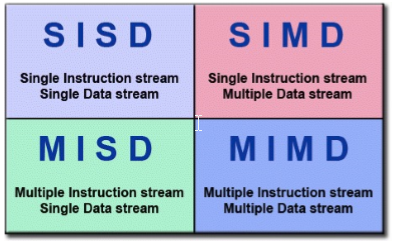
\includegraphics[width=\linewidth,keepaspectratio=true]{Images/flynn}
	\end{minipage}%%% to prevent a space
	\begin{minipage}{0.2\textwidth}
		SISD is used in a single core.\\
		SIMD für zB GPU\\
		MISD für failsafe Systeme\\
		MIMD für Clusters
	\end{minipage}
\end{minipage}

\subsection{Memory}
Es gibt grundsätzlich folgende Memory Typen:
\begin{enumerate}[nosep]
	\item Shared Memory
	\item Distributed Memory
	\item Hybrid Distributed-Shared Memory
\end{enumerate}

Oft ist der Memory-Throughput der Bottleneck. In modernen CPU, welche nach \textbf{Neumann Computer Architecture} gebaut sind, sind Instruktion und Data Memory am gleichen Bus angebunden. Im Gegensatz zu Embedded Geräten, welche nach \textbf{Harvard Architecture} zwei Buse existieren.
~\\~\\
Um diesen Problem entgegenzuwirken wird von UMA (Uniform memory access) zu NUMA (Non-Uniform memory access) gewechselt. Der Bus Interconnect verbindet muss sehr schnell sein (100GBit/s Ethernet), dies wird mit dem \textbf{MPI} umgesetzt. 
\begin{center}
	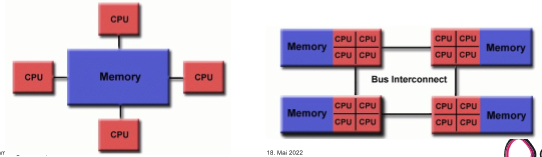
\includegraphics[width=0.6\columnwidth]{Images/uma}
\end{center}


\subsection{MPI API}
Die Anzahl Aktors sind fix beim Starten und können nicht zur Laufzeit geändert werden. Es gibt zudem auch kein Data Races, weil kein Shared Memory zwischen den Prozessen existiert.
\begin{tabular}{p{4cm}|p{4cm}}
	\textbf{MPI\_Barrier} & Warten, bis alle Prozesse Barrier erreicht haben \\
	\textbf{MPI\_Allreduce} & Aggregation von Teilresultaten zwischen Prozessoren, jeder erhält Gesamtresultat als Rückgabewert (inkl Broadcast) \\
	\textbf{MPI\_Reduce} & Aggregation von Teilresultaten zwischen Prozessoren, nur ein Prozess (rank) erhält Gesamtresultat \\
	\textbf{MPI\_Bcast} & Sendet Nachricht an mehrere Targets\\
	\textbf{MPI\_Send} & Sendet blockierend an Target \\
	\textbf{MPI\_Recv} & Empfängt blockierend von Sender \\
\end{tabular}

\subsubsection{Demo}
Der folgende Code muss mit \textit{mpicc -o app demo.c} kompiliert und mit \textit{mpiexec -n 32 app} ausgeführt werden. Dabei werden 32 von der gleichen Applikation gestartet verteilt auf den verfügbaren CPU.
\begin{lstlisting}
	#include <stdio.h> 
	#include "mpi.h" 
	
	int main(int argc, char* argv[]) {
		MPI_Init(&argc, &argv);
		
		int rank, size;
		MPI_Comm_rank(MPI_COMM_WORLD, &rank);
		MPI_Comm_size(MPI_COMM_WORLD, &size);
		char name[MPI_MAX_PROCESSOR_NAME];
		int len;
		MPI_Get_processor_name(name, &len);
		printf("Hello cluster from process %i on %s\n", rank, name);
		
		if (rank == 0) {
			int value = rand();
			for (int to = 1; to < size; to++) {
				MPI_Send(&value, 1, MPI_INT, to, 0 , MPI_COMM_WORLD);
			}
		} else {
			int value;
			MPI_Recv(&value, 1, MPI_INT, 0, 0, MPI_COMM_WORLD, MPI_STATUS_IGNORE);
			printf("%i received by %i", value, rank);
		}
		
		MPI_Finalize();
		
		return 0;
	}
\end{lstlisting}

\subsection{openMP}
OpenMP verwaltet Threads in einer MPI Umgebung, das zu einem Hybrid Model zwischen Threads und Nodes führt.

Das folgende Programm startet \textbf{OMP\_NUM\_THREADs} Threads pro Programm sobald pragma erreicht ist und führt den Folgenden Block parallel aus.
\begin{lstlisting}
#include <stdio.h>
#include <omp.h>
	
int main(int argc, char* argv[]) {
	const int np = omp_get_max_threads();
	printf("OpenMP with threads %d\n", np);
	
#pragma omp parallel
	{
		const int id = omp_get_thread_num();
		printf("Hello from thread %d\n", id);
	}

	return 0;
}
\end{lstlisting}

Um eine For-Schleife Parallel auszuführen kann ein \textit{for} nach dem pragma hinzugefügt werden. Variable A ist für jeden Thread private, B wird über alle Threads geshared (aber nicht synchronisiert)

\begin{lstlisting}
long hits = 0;
long i;
double x,y;
long count_hits(long trails) {
	#pragma omp parallel
	{
	#pragma omp parallel for reduction(+:hits) private (x,y)
		for (i = 0; i < trails; ++i) {
			x = random_double();
			y = random_double();
			if (x*x + y*y <= 1) hits++;
		}
	}
	return hits;
}	
\end{lstlisting}